\documentclass[11pt]{article}
\usepackage[margin=1in]{geometry}
\usepackage{amsmath,amssymb,amsthm}
\usepackage{graphicx}
\usepackage[colorlinks=true,linkcolor=blue,citecolor=blue,urlcolor=blue]{hyperref}
\newtheorem{theorem}{Theorem}[section]
\newtheorem{lemma}[theorem]{Lemma}
\newtheorem{corollary}[theorem]{Corollary}
\newtheorem{definition}[theorem]{Definition}
\newtheorem{assumption}[theorem]{Assumption}
\newtheorem{hypothesis}[theorem]{Hypothesis}
\newtheorem{conjecture}[theorem]{Conjecture}
\theoremstyle{remark}
\newtheorem{remark}[theorem]{Remark}
\newcommand{\Tr}{\operatorname{Tr}}

\title{From Static Recoverability to Maintenance Power:\\
A Typed Pipeline with $\omega = 0$ Obstructions\\
{\normalsize Version 2}}
\author{Lluis Eriksson\\ Independent Researcher\\ \texttt{lluiseriksson@gmail.com}}
\date{January 2026 (v1); July 2026 (v2)}

\begin{document}
\maketitle

\begin{abstract}
We study when geometric separation in gapped quantum systems yields a
genuine reduction in thermodynamic resources required to maintain coherence
against uncontrolled open-system dynamics. Our analysis separates three
layers. First, in a regularized Gaussian split regime motivated by
algebraic QFT, we state an explicit static reconstruction bound: collar
suppression of vacuum cross-correlations enables approximate state recovery
via a conditional-reattachment covariance rule with fidelity error
controlled by a cross-block recovery norm. Second, we show why static
recoverability does not automatically imply suppression of dynamical decay
rates: fixed-point structure and Bohr-zero ($\omega = 0$) channels can
generate obstructions invisible to static clustering alone. We formalize
this using an exact $\omega = 0$ Dirichlet identity and implement
finite-size commutator-witness diagnostics in the transverse-field Ising
chain, finding no evidence of a size-independent $\omega = 0$ floor in that
benchmark regime for tested sizes. Third, we give an autocontained
finite-dimensional core linking coherence loss to incremental maintenance
power under an explicit battery-assisted thermal-operations model with
paired strategies, and we state a typed rate-inheritance hypothesis
identifying precisely what additional dynamical input is required to
propagate collar suppression into power suppression. We conclude with a
Type III blueprint. \emph{v2 corrects two points and adds verification:}
(i) the recovery rule of the static layer is conditional reattachment --
\emph{not} the Petz map for correlated Gaussian references (aligned with
2601.0007 v2 and 2512.0060 v2), with an explicit admissibility hypothesis;
(ii) the v1 work-cost bookkeeping (its Eq.~(25)) carried a sign error --
the work cost is the battery free-energy \emph{decrease} -- which made v1's
one-step work lemma false as printed (random energy-conserving unitaries
violate it in 57/100 draws) while its own proof chain and everything
downstream hold verbatim with the corrected sign; this is the same error
class repaired in 2512.0061 v2. v2 further adds a GNS/KMS convention
bridge to the companion witness papers, series positioning, an updated
status of the rate-inheritance hypothesis, and a verification suite.
\end{abstract}

\section{Introduction}
Geometric separation in gapped many-body systems suppresses static
correlations, motivating the expectation that thick buffers reduce
cross-region influence. A distinct operational question is dynamical: even
if a global state is recoverable from local data, what resources are
required to keep a target state stable under uncontrolled open-system
dynamics? This paper isolates a frequent logical pitfall: static locality
controls an \emph{amplitude}, whereas maintenance cost is governed by
\emph{rates}. Our contribution is a typed pipeline separating static
recoverability from dynamic rate control, identifying the unique missing
hinge (rate inheritance on a family), and clarifying the role of
$\omega = 0$/fixed-point obstructions.

\paragraph{Series positioning (added in v2).} This note is the integrative
closure of the 2601 block: the static layer instantiates 2601.0007
\cite{S0007} (finite-mode core of 2512.0060 \cite{S0060}); the
$\omega = 0$ obstruction and witnesses develop 2601.0022/0023
\cite{S0022, S0023}; the maintenance bound is the paired-strategy theorem
of 2512.0061 v2 \cite{S0061}, reproved here self-contained; the typed
rate-inheritance hypothesis is the family-level version of the hinge
formulated in 2512.0072 \cite{S0072}, stress-tested in 2512.0070
\cite{S0070}, proved in the quasi-free class in 2512.0064 \cite{S0064},
and reduced to a Dirichlet comparison in 2601.0020 \cite{S0020}; the
Type III blueprint points at 2512.0101 \cite{S0101}.

\section{Setup: conditional expectations, coherence functionals, and
operational families}
Let $\mathcal{H}$ be finite-dimensional, $H_S$ with spectral projectors
$\{\Pi_n\}$, $\beta := 1/(k_B T)$, $\sigma := e^{-\beta H_S}/
\Tr(e^{-\beta H_S})$, and $T_t = e^{t\mathcal{L}_*}$ an uncontrolled GKLS
semigroup with $\mathcal{L}_*[\sigma] = 0$.
\begin{definition}[Coherence relative to a conditional expectation]
For a $\sigma$-preserving conditional expectation $E$ with predual $E_*$,
$C_E(\rho) := S(\rho\,\|\,E_*[\rho])$. Instance 1 (law-grade): energy
pinching $\Delta[A] = \sum_n \Pi_n A \Pi_n$. Instance 2 (static,
geometric): a vacuum-preserving split expectation $E_{\rm split}$ in a
split configuration $\mathcal{O}_1 \Subset \mathcal{O}_2$ of collar width
$r$.
\end{definition}
Loss rate: $\dot C_{E,\rm loss}(\rho) := -\frac{d}{dt}C_E(T_t\rho)|_{t=0}$;
local rate $r_E(\rho) := \dot C_{E,\rm loss}(\rho)/C_E(\rho)$ for
$C_E(\rho) > 0$; typed envelopes $r^\downarrow_E(r) := \inf_{\rho \in
\mathcal{F}_r} r_E(\rho)$ and $r^\uparrow_E(r) := \sup_{\rho \in
\mathcal{F}_r} r_E(\rho)$ on an operational family $\mathcal{F}_r$ of
locally prepared states ($\rho = \Lambda_A(\sigma)$, $\Lambda_A$ with
Stinespring dilation localized in $A$) with energy budget, optional
coherence budget, and fixed-point exclusion
$\|\rho - E_{\rm fix,*}[\rho]\|_1 \ge \delta_{\rm fix}$, where
$E_{\rm fix,*}$ is the ergodic mean of $T_t$.

\section{Static layer: quantitative recoverability from collar suppression
(Gaussian split regime; terminology corrected in v2)}
With centered quasi-free covariances $\Gamma, \Gamma_0$ in block form,
vacuum correlation factor $\eta_{\rm vac} := \|A_0^{-1/2} X_0
B_0^{-1/2}\|_{\rm op}$ and perturbation $\delta_X := \|A_0^{-1/2}(X - X_0)
B_0^{-1/2}\|_{\rm op}$, the \emph{conditional-reattachment} covariance rule
is
\[
\tilde A = A, \qquad \tilde X = A A_0^{-1} X_0, \qquad
\tilde B = B_0 + X_0^T A_0^{-1}(A - A_0)A_0^{-1} X_0,
\qquad \Delta^{(12)} := X - \tilde X .
\]
\begin{remark}[Terminology corrected in v2]
\label{rem:petzfix}
v1 called this rule ``Petz recovery in block form.'' Per 2601.0007 v2
\cite{S0007} (aligned with the repaired Proposition 2.14 of 2512.0060 v2
\cite{S0060}), the rule is conditional reattachment: it agrees with the
Petz output only for factorized references ($X_0 = 0$); for correlated
references the Petz map does not preserve the input marginal. All uses
below are of the explicit covariance rule on its admissible domain
($\tilde\Gamma + \frac{i}{2}\Omega \succeq 0$).
\end{remark}
\begin{theorem}[Gaussian clustering--recovery bridge (static; imported)]
\label{thm:static}
Under quasi-free regularity, coercivity of $A$ relative to $A_0$,
cross-correlation control, $\|K\|_{\rm op} \le 1/2$, and admissibility of
$\tilde\Gamma$, the reattached state $\tilde\omega$ satisfies
$1 - F(\omega, \tilde\omega) \le C(\epsilon, \eta_{\rm vac}, \delta)\,
\|\Delta^{(12)}\|_{\rm HS}^2$, with prefactor controlled by $\epsilon$ and
the correlation denominator $1 - \epsilon^{-1}(\eta_{\rm vac} +
\delta)^2$. See \cite{S0007} for the proved quantitative version
(quadratic+quartic, with certified constants).
\end{theorem}
\begin{remark}[Static only]
Theorem~\ref{thm:static} is a static reconstruction guarantee; it implies
nothing about dynamical rates.
\end{remark}

\section{The $\omega = 0$ obstruction and witness diagnostics}
With $S(0) := \sum_n \Pi_n S \Pi_n$ and an $\omega = 0$ Davies channel
$\mathcal{L}_0(O) = \gamma(0)(S(0)OS(0) - \tfrac12\{S(0)^2, O\})$, we use
the $\sigma$-weighted (GNS) inner product $\langle A, B\rangle_\sigma :=
\Tr(A^\dagger \sigma B)$, matching the numerical diagnostics (for Pauli
strings $\|O\|^2_{2,\sigma} = 1$).
\begin{lemma}[Exact $\omega = 0$ Dirichlet identity (GNS)]
If $[S(0), \sigma] = 0$, then $\mathcal{E}^{(0)}_\sigma(O) =
\tfrac{\gamma(0)}{2}\|[S(0), O]\|^2_{2,\sigma}$ for all $O$.
\end{lemma}
\begin{remark}[Convention bridge (added in v2)]
\label{rem:conv}
The companions 2601.0022/0023 \cite{S0022, S0023} state the same identity
in the \emph{KMS} inner product $\Tr(\sigma^{1/2}A^\dagger\sigma^{1/2}B)$;
the proof only uses $[S(0), \sigma] = 0$ and holds in both. The optimized
witness values differ numerically between conventions (suite benchmark,
TFIM $N = 8$: ratio GNS/KMS $\approx 1.15$ at $\epsilon = 1$, $1.24$ at
$\epsilon = 2$), so cross-paper comparisons of $R_{\rm opt}$ must fix the
convention. This paper's numbers are GNS throughout.
\end{remark}
Witness families: $R^{(k)}_{\rm opt}(\epsilon; N) := \max_O
\|[S(0),O]\|^2_{2,\sigma}/\|O\|^2_{2,\sigma}$ over one-site and two-site
Pauli families at distance $\epsilon$, certifying
$\kappa^{(k)}_{\rm wit} = \tfrac{\gamma(0)}{2}R^{(k)}_{\rm opt}$ within the
family.
\begin{remark}[Consistency with the companions (added in v2)]
\label{rem:trend}
Figure~\ref{fig:sweep} shows $R_{\rm opt}$ \emph{decreasing with $N$} at
fixed $\epsilon$: no evidence of a size-independent $\omega = 0$ floor in
this benchmark. This refines -- and does not contradict -- 2601.0022/0023,
which certify a strictly positive floor \emph{mechanism at fixed $N$}: the
mechanism is real (and switches off for couplings with vanishing
$\omega = 0$ component, per the 0022 v2 null case), while its
$N$-dependence in this benchmark suggests it need not survive the
thermodynamic limit for this coupling family. The suite reproduces the
decreasing trend ($N \in \{6, 8, 10\}$, $\epsilon \in \{1, 2\}$).
\end{remark}
\begin{figure}[h]\centering
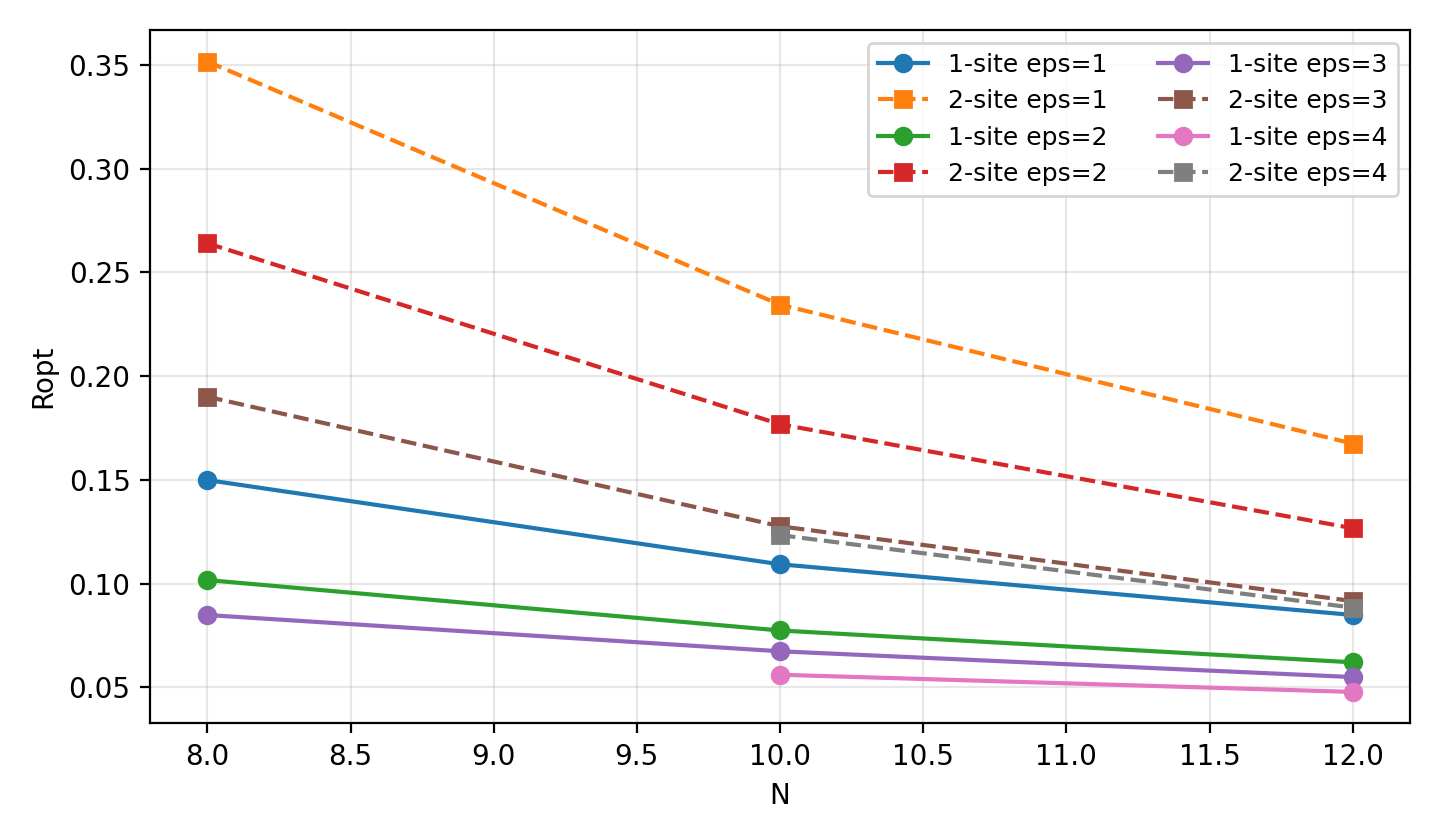
\includegraphics[width=0.8\textwidth]{fig1_witness_sweep.png}
\caption{Optimized $\omega = 0$ commutator witnesses in the TFIM ($J = 1$,
$h = 1.5$, $\beta = 1$). Solid: one-site family; dashed: adjacent two-site
family. Both decrease with $N$ at fixed $\epsilon$ for $N \le 12$.}
\label{fig:sweep}
\end{figure}

\section{Thermodynamic control model and the power bound (sign corrected
in v2)}
Battery-assisted thermal operations: $\Phi_{SW}(\cdot) = \Tr_B[U(\cdot
\otimes \gamma_B)U^\dagger]$ with $[U, H_S + H_B + H_W] = 0$; battery
free energy $F_\beta(\omega_W) := k_B T\, S(\omega_W\|\gamma_W)$.
\begin{definition}[Work cost; sign corrected in v2]
\label{def:work}
For a battery process $\omega_W \mapsto \omega'_W$, the work
\emph{expenditure} is
\[
W := F_\beta(\omega_W) - F_\beta(\omega'_W),
\]
the battery free-energy \emph{decrease}. (v1's Eq.~(25) defined $W$ with
the opposite sign, which renders its one-step lemma false as printed: the
suite exhibits violations in 57/100 random energy-conserving unitaries,
while the corrected sign yields 0/100. This is the same error class as the
work-sign bug repaired in 2512.0061 v2 \cite{S0061}.)
\end{definition}
Instantaneous maintenance and \emph{paired} incremental power
$P_{\rm extra}(\rho)$ are defined as in v1 (paired strategies maintaining
$\rho$ and $\Delta[\rho]$ with the same bath model and initial battery
state; one never subtracts unrelated infima).
\begin{lemma}[One-step work lower bound, corrected sign]
\label{lem:work}
For $\Phi_{SW}$ as above mapping $\rho \otimes \omega_W$ to a state with
marginals $\rho'$, $\omega'_W$:
$W \ge F^S_\beta(\rho') - F^S_\beta(\rho)$, with $F^S_\beta(\rho) := k_B T
\, S(\rho\|\sigma) + {\rm const}$.
\end{lemma}
\begin{proof}
Energy conservation gives $U\Gamma U^\dagger = \Gamma$ for $\Gamma =
\sigma \otimes \gamma_B \otimes \gamma_W$. Monotonicity of relative
entropy under $\Tr_B U(\cdot)U^\dagger$ plus the chain rule with
$I(S{:}W) \ge 0$ yield
$S(\rho\|\sigma) + S(\omega_W\|\gamma_W) \ge S(\rho'\|\sigma) +
S(\omega'_W\|\gamma_W)$, i.e.\ total nonequilibrium free energy does not
increase. Rearranged: $F_\beta(\omega_W) - F_\beta(\omega'_W) \ge
F^S_\beta(\rho') - F^S_\beta(\rho)$, which is the claim with the corrected
sign convention. (v1 derived exactly this display -- its Eq.~(36) -- and
then transcribed it with the inverted work sign.)
\end{proof}
\begin{assumption}[Energy covariance of the drift]
\label{ass:cov}
$\Delta[T_t(\rho)] = T_t(\Delta[\rho])$ (holds for Davies/secular
generators; verified in the suite).
\end{assumption}
\begin{theorem}[Incremental maintenance power lower bound (paired
strategies)]
\label{thm:power}
Under the maintenance model, Definition~\ref{def:work}, and
Assumption~\ref{ass:cov}, if paired strategies exist for $\rho$ and
$\Delta[\rho]$, then
$P_{\rm extra}(\rho) \ge k_B T\, \dot C_{\Delta,\rm loss}(\rho)$.
\end{theorem}
\begin{proof}
Verbatim as in v1 with $W$ of Definition~\ref{def:work}: apply
Lemma~\ref{lem:work} to both maintenance steps, subtract the paired
inequalities, use the pinching Pythagoras identity
$S(\rho\|\sigma) = S(\rho\|\Delta[\rho]) + S(\Delta[\rho]\|\sigma)$ and
Assumption~\ref{ass:cov}, divide by $\delta t$ and pass to the limit.
\end{proof}

\section{Main results: finite-dimensional core and Type III blueprint}
\begin{corollary}[Typed family lower bound]
For $\rho \in \mathcal{F}_r$ with $C_\Delta(\rho) > 0$, with
$P_{\rm extra}$ the \emph{paired} incremental power of
Theorem~\ref{thm:power}:
$P_{\rm extra}(\rho) \ge k_B T\, r_\Delta(\rho)\, C_\Delta(\rho) \ge
k_B T\, r^\downarrow_\Delta(r)\, C_\Delta(\rho)$.
\end{corollary}
\begin{hypothesis}[Typed rate inheritance on $\mathcal{F}_r$; status
updated in v2]
\label{hyp:rip}
On $\mathcal{F}_r$, $r^\downarrow_\Delta(r) > 0$ with a collar-dependent
envelope (e.g.\ $r^\downarrow_\Delta(r) \gtrsim e^{-\alpha r}$ up to
polynomial prefactors), and fixed-point/$\omega = 0$ mechanisms do not
induce a collar-independent floor in the relevant regime. \emph{Status in
the series:} proved exactly in the quasi-free local-sink class
\cite{S0064}; failure scenario realized within the secular Davies class
\cite{S0070} (with the nonlocality caveat there); reduced to an explicit
bulk--collar Dirichlet comparison in \cite{S0020}; the $\omega = 0$
no-floor input is supported in the TFIM benchmark by
Remark~\ref{rem:trend} at tested sizes.
\end{hypothesis}
\begin{corollary}[Collar-dependent power suppression (conditional)]
Assuming Hypothesis~\ref{hyp:rip} and $C_\Delta \ge C_0 > 0$ on
$\mathcal{F}_r$, the paired incremental power satisfies
$\inf_{\rho \in \mathcal{F}_r} P_{\rm extra}(\rho)
\gtrsim k_B T\, r^\downarrow_\Delta(r)\, C_0$.
\end{corollary}
\begin{conjecture}[Typed pipeline in AQFT (blueprint)]
As in v1: with a split inclusion of collar width $r$, static residue
$C_{E_{\rm split}}(\omega) := S_{\rm Araki}(\omega\|\omega \circ
E_{\rm split})$, a physically specified dissipative dynamics and a
well-posed maintenance notion, a Type III analogue of
Hypothesis~\ref{hyp:rip} yields, for the paired incremental power,
$P_{\rm extra}(\omega) \gtrsim k_B T\,
r^\downarrow_\Delta(r)\, C_{E_{\rm split}}(\omega)$ on a typed fast-sector
family. The CMI route to the static side is 2512.0101 \cite{S0101}.
\end{conjecture}

\section{Verification suite (added in v2)}
\label{sec:verif}
\texttt{verification/2601-0031/verify\_2601\_0031.py}: (1) the
$\omega = 0$ identity in the GNS convention (machine precision); (2) the
GNS/KMS bridge of Remark~\ref{rem:conv}; (3) the decreasing-with-$N$
witness trend ($N \in \{6,8,10\}$, both $\epsilon$); (4) the pinching
Pythagoras identity (exact); (5) the work-sign refutation/repair of
Definition~\ref{def:work} (57/100 violations with v1's sign; 0/100
corrected) on random energy-conserving unitaries over
$S \otimes B \otimes W$; (6) Assumption~\ref{ass:cov} for a secular Davies
generator (exact). The Figure~\ref{fig:sweep} script of v1's appendix is
relocated to the same directory.

\section{Conclusion}
Geometry buys recoverability (Theorem~\ref{thm:static}); it does not buy
efficiency freely: maintenance is governed by rate envelopes vulnerable to
fixed-point and $\omega = 0$ obstructions that static clustering cannot
rule out. The missing dynamical hinge is explicit
(Hypothesis~\ref{hyp:rip}, with its series status), and the witness
diagnostics delineate when ``isolation implies stability'' becomes
thermodynamically valid.

\section*{Note added in v2}
Two corrections, both verified in the suite, plus positioning. (1)
\emph{Terminology/admissibility (static layer):} ``Petz'' $\to$
conditional reattachment per 2601.0007 v2 and 2512.0060 v2
(Remark~\ref{rem:petzfix}), with the admissibility hypothesis stated. (2)
\emph{Work-sign error:} v1's Eq.~(25) inverted the work-cost sign, making
its one-step lemma false as printed; the corrected bookkeeping
(Definition~\ref{def:work}) restores it, and Theorem~\ref{thm:power} holds
verbatim -- v1's own proof chain (its Eq.~(36)) already established the
corrected display. Same error class as 2512.0061 v1 (repaired in its v2).
(3) Additions: GNS/KMS convention bridge (Remark~\ref{rem:conv});
consistency remark with the fixed-$N$ floor mechanism of 2601.0022/0023
(Remark~\ref{rem:trend}); series citations (v1 cited no companion);
updated status of Hypothesis~\ref{hyp:rip}; verification suite; appendix
script relocated.

\begin{thebibliography}{14}
\bibitem{Davies} E. B. Davies, Commun. Math. Phys. \textbf{39} (1974)
91--110.
\bibitem{Spohn} H. Spohn, J. Math. Phys. \textbf{19} (1978) 1227--1230.
\bibitem{Petz} D. Petz, Commun. Math. Phys. \textbf{105} (1986) 123--131.
\bibitem{BBP} L. Banchi, S. L. Braunstein, S. Pirandola, Phys. Rev. Lett.
\textbf{115} (2015) 260501.
\bibitem{FR} O. Fawzi, R. Renner, Commun. Math. Phys. \textbf{340} (2015)
575--611.
\bibitem{S0060} L. Eriksson, ai.viXra:2512.0060 (2025; v2 2026).
\bibitem{S0061} L. Eriksson, ai.viXra:2512.0061 (2025; v2 2026).
\bibitem{S0064} L. Eriksson, ai.viXra:2512.0064 (2025; v2 2026).
\bibitem{S0070} L. Eriksson, ai.viXra:2512.0070 (2025; v2 2026).
\bibitem{S0072} L. Eriksson, ai.viXra:2512.0072 (2025; v2 2026).
\bibitem{S0101} L. Eriksson, ai.viXra:2512.0101 (2025; v2 2026).
\bibitem{S0007} L. Eriksson, ai.viXra:2601.0007 (2026; v2 2026).
\bibitem{S0020} L. Eriksson, ai.viXra:2601.0020 (2026; v2 2026).
\bibitem{S0022} L. Eriksson, ai.viXra:2601.0022 (2026; v2 2026);
2601.0023 (2026; v2 2026).
\bibitem{S0023} L. Eriksson, ai.viXra:2601.0023 (2026; v2 2026).
\end{thebibliography}
\end{document}
